\documentclass[aspectratio=169]{beamer}
\usepackage{tikz}
\usepackage{fancyvrb}
\usepackage{xcolor}
\title{Asymmetric Cryptography Part 2\\RPISEC}
\date{November 1, 2019}
\author{Avi Weinstock (\Verb|aweinstock|),\\ Jacques Becker (\Verb|off\_by\_1\_error|), Ethan Wright (\Verb|eth4|)}

\definecolor{rpisecbgcolor}{RGB}{21, 24, 32} % 151820
\definecolor{cybercyan}{RGB}{42, 171, 219} % 2aabdb
\definecolor{cybergreen}{RGB}{106, 220, 169} % 6adca9
\definecolor{cyberpink}{RGB}{248, 106, 140} % f86a8c

\setbeamercolor{normal text}{fg=white}
\setbeamercolor{frametitle}{fg=cybercyan}
\setbeamercolor{title}{fg=cybercyan}
\setbeamercolor{structure}{fg=cybercyan}

%>>> [0x15,0x18,0x20]
%[21, 24, 32]
% convert rpisec_background.png -alpha set -fill '#15182080' -draw 'rectangle 0 0 1090 1216' rpisec_background2.png
% convert probable_prime.png -alpha set -fill '#151820c0' -draw 'rectangle 0 0 414 836' probable_prime2.png
\usebackgroundtemplate{
\colorbox{rpisecbgcolor}{\raisebox{1pt}[\paperheight][\depth]{\hspace{0.6\paperwidth}
%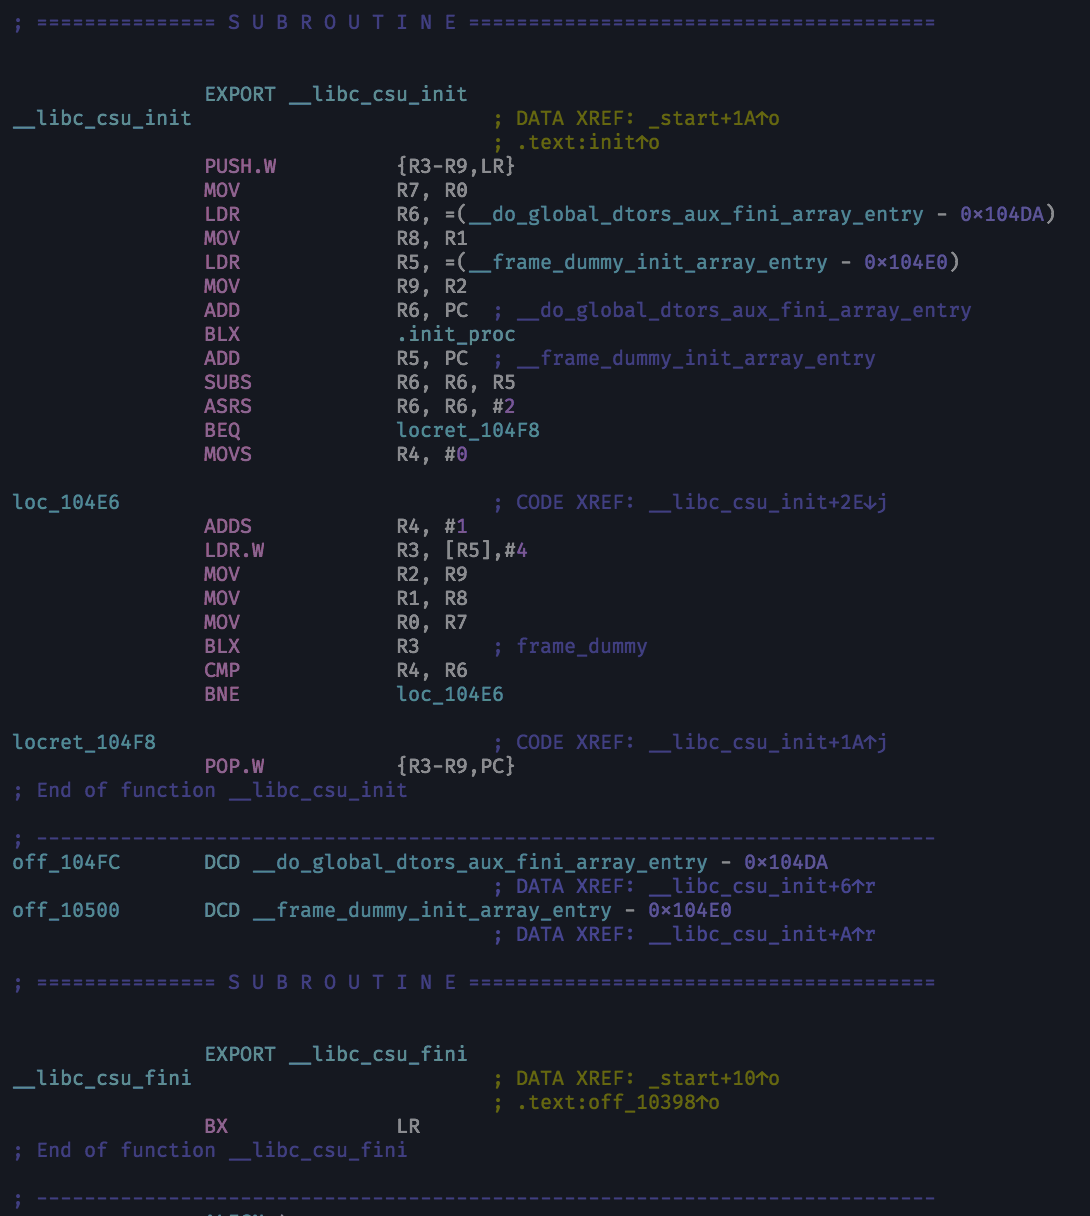
\includegraphics[width=0.4\paperwidth, height=\paperheight]{rpisec_background2.png}
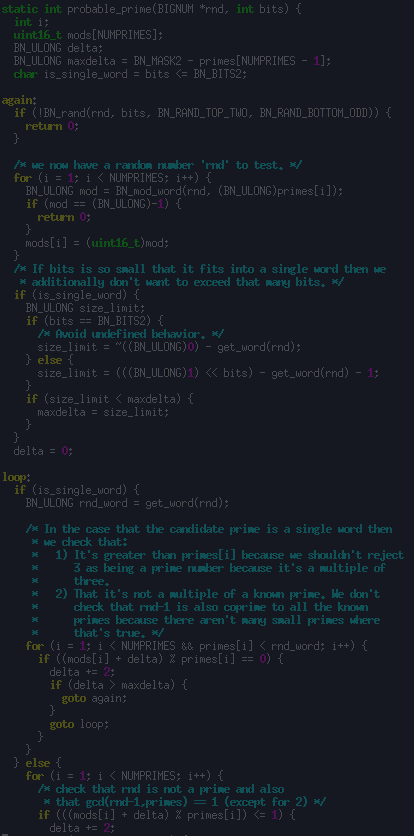
\includegraphics[width=0.4\paperwidth, height=\paperheight]{../rsa_2019_10_29/probable_prime2.png}
}}
}

\begin{document}
\maketitle

\begin{frame}[fragile]
\frametitle{RSA Recap}
\begin{Verbatim}[fontsize=\scriptsize]
from codecs import encode
from gmpy import invert, next_prime
import os
d = 0
while d == 0:
    p = next_prime(int(encode(os.urandom(1024/8), 'hex'), 16))
    q = next_prime(int(encode(os.urandom(1024/8), 'hex'), 16))
    n = p * q
    phi = (p - 1) * (q - 1)
    e = 65537
    d = invert(e, phi)

message = int(encode('hello', 'hex'), 16)
ciphertext = pow(message, e, n)
assert pow(ciphertext, d, n) == message
\end{Verbatim}
\end{frame}

\begin{frame}[fragile]
\frametitle{Example RSA encryption/decryption}
\begin{minipage}{0.3\textwidth}
\begin{itemize}
\item $n = p * q$
\item $\varphi(n) = (p-1)*(q-1)$
\item $e * d \equiv 1\hspace{1mm}(\text{mod } \varphi(n))$
\item $\verb|encrypt|(x) = x^e \% n$
\item $\verb|decrypt|(x) = x^d \% n$
\item $\verb|pow(x, k, n)| = x^k \% n$
\end{itemize}
\end{minipage}
\begin{minipage}{0.6\textwidth}
\begin{itemize}
\item<1-> Public: $(n, e) = (667, 3)$
\item<1-> Message \verb|"hi"|, encoded as $7*26+8 = 190$
\item<1-> \verb|pow(190, 3, 667) == 239|
\item<2> Private: $(p, q, d) = (23, 29, 411)$
\item<2> \verb|(3 * 411) % (22 * 28) == 1|
\item<2> \verb|pow(239, 411, 23*29) == 190|
\end{itemize}
\end{minipage}
\end{frame}

\begin{frame}[fragile]
\frametitle{Why to use e = 65537}
\begin{itemize}
\item $2^{16}+1 = 65537_{10} = 10001_{16} = 10000000000000001_2$
\item It's prime, so $\verb|invert|(65537, \varphi(n))$ is more likely to exist
\item It mitigates multiple attacks:
\begin{itemize}
\item Cube root
\item Hastad's broadcast
\item Coppersmith's short pad
\end{itemize}
\item Since it only has 2 bits set, it's efficient to compute via repeated squaring:
$m^{2^{16}+1} = m^{2^{16}}*m = (m^{2^8}*m^{2^8})*m = ((m^{2^4}*m^{2^4})*(m^{2^4}*m^{2^4}))*m = \hdots$
\end{itemize}
\end{frame}

\begin{frame}[fragile]
\frametitle{Extended Euclidean Algorithm}
\begin{itemize}
\item \VerbatimInput[fontsize=\scriptsize]{eea.py}
\end{itemize}
\end{frame}

\begin{frame}[fragile]
\frametitle{Handwritten CRT Presentation - 1/4}
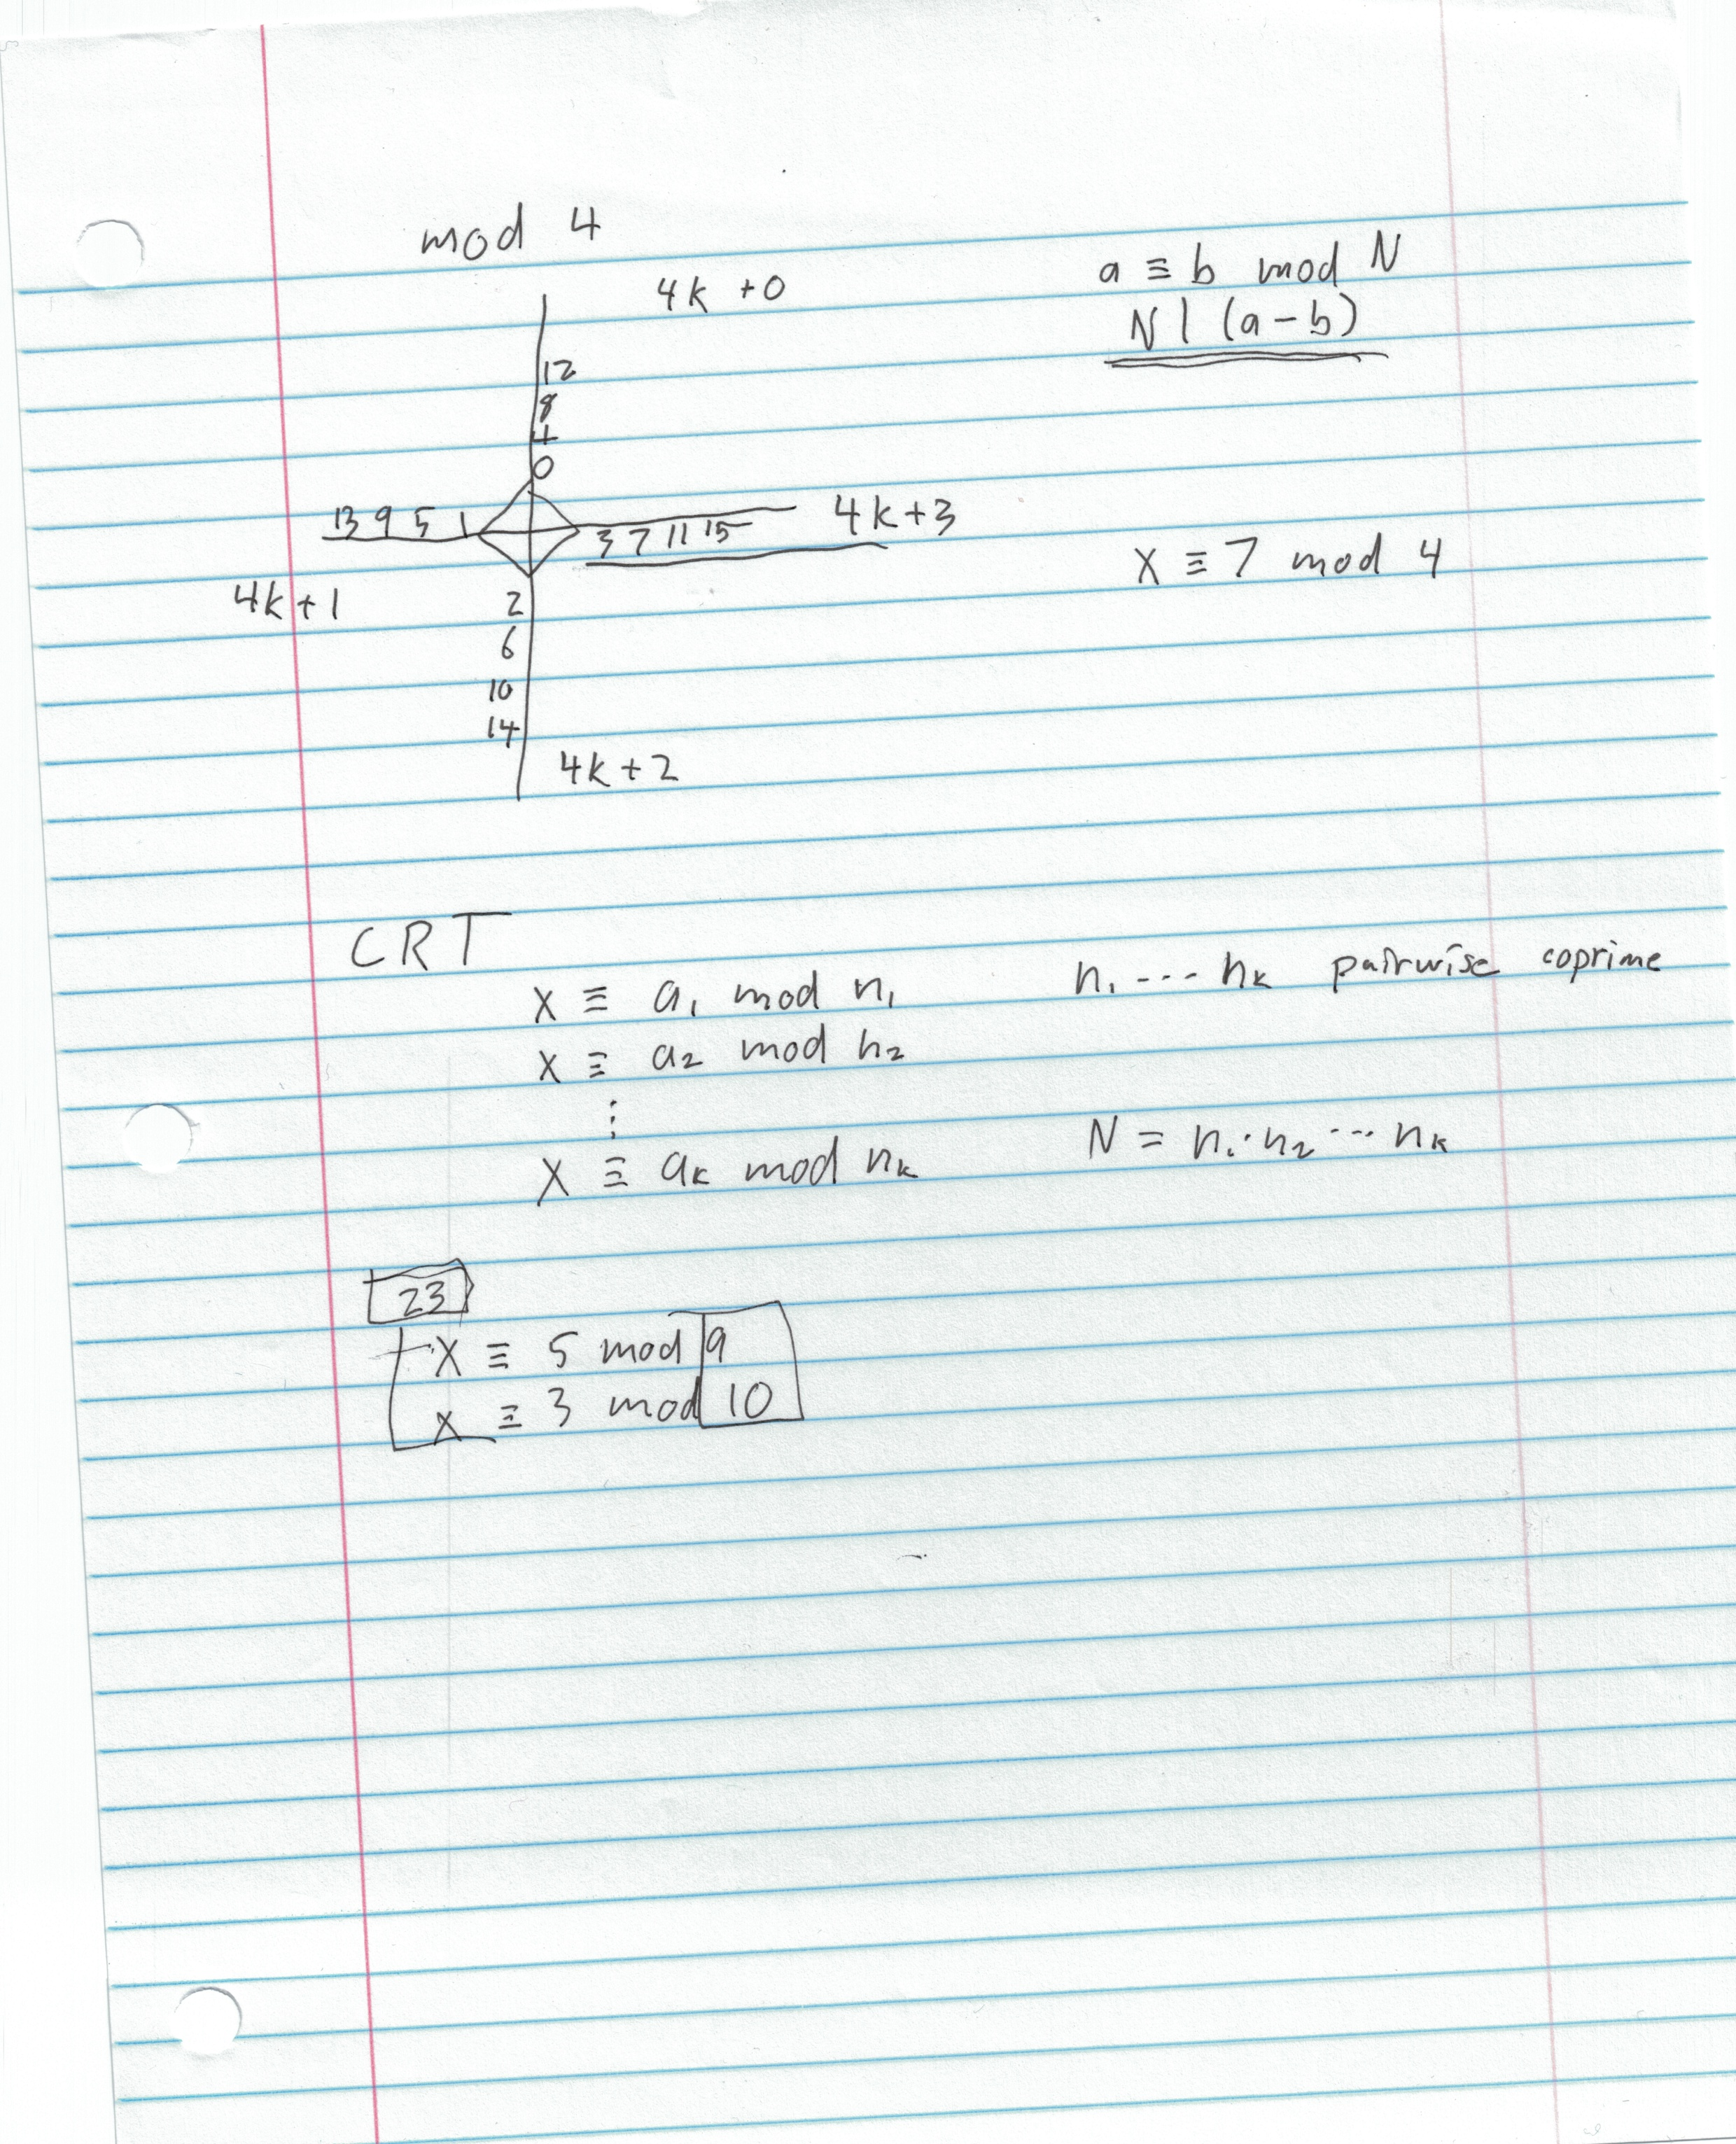
\includegraphics[height=0.8\paperheight]{jacques_page1.jpg}
\end{frame}
\begin{frame}[fragile]
\frametitle{Handwritten CRT Presentation - 2/4}
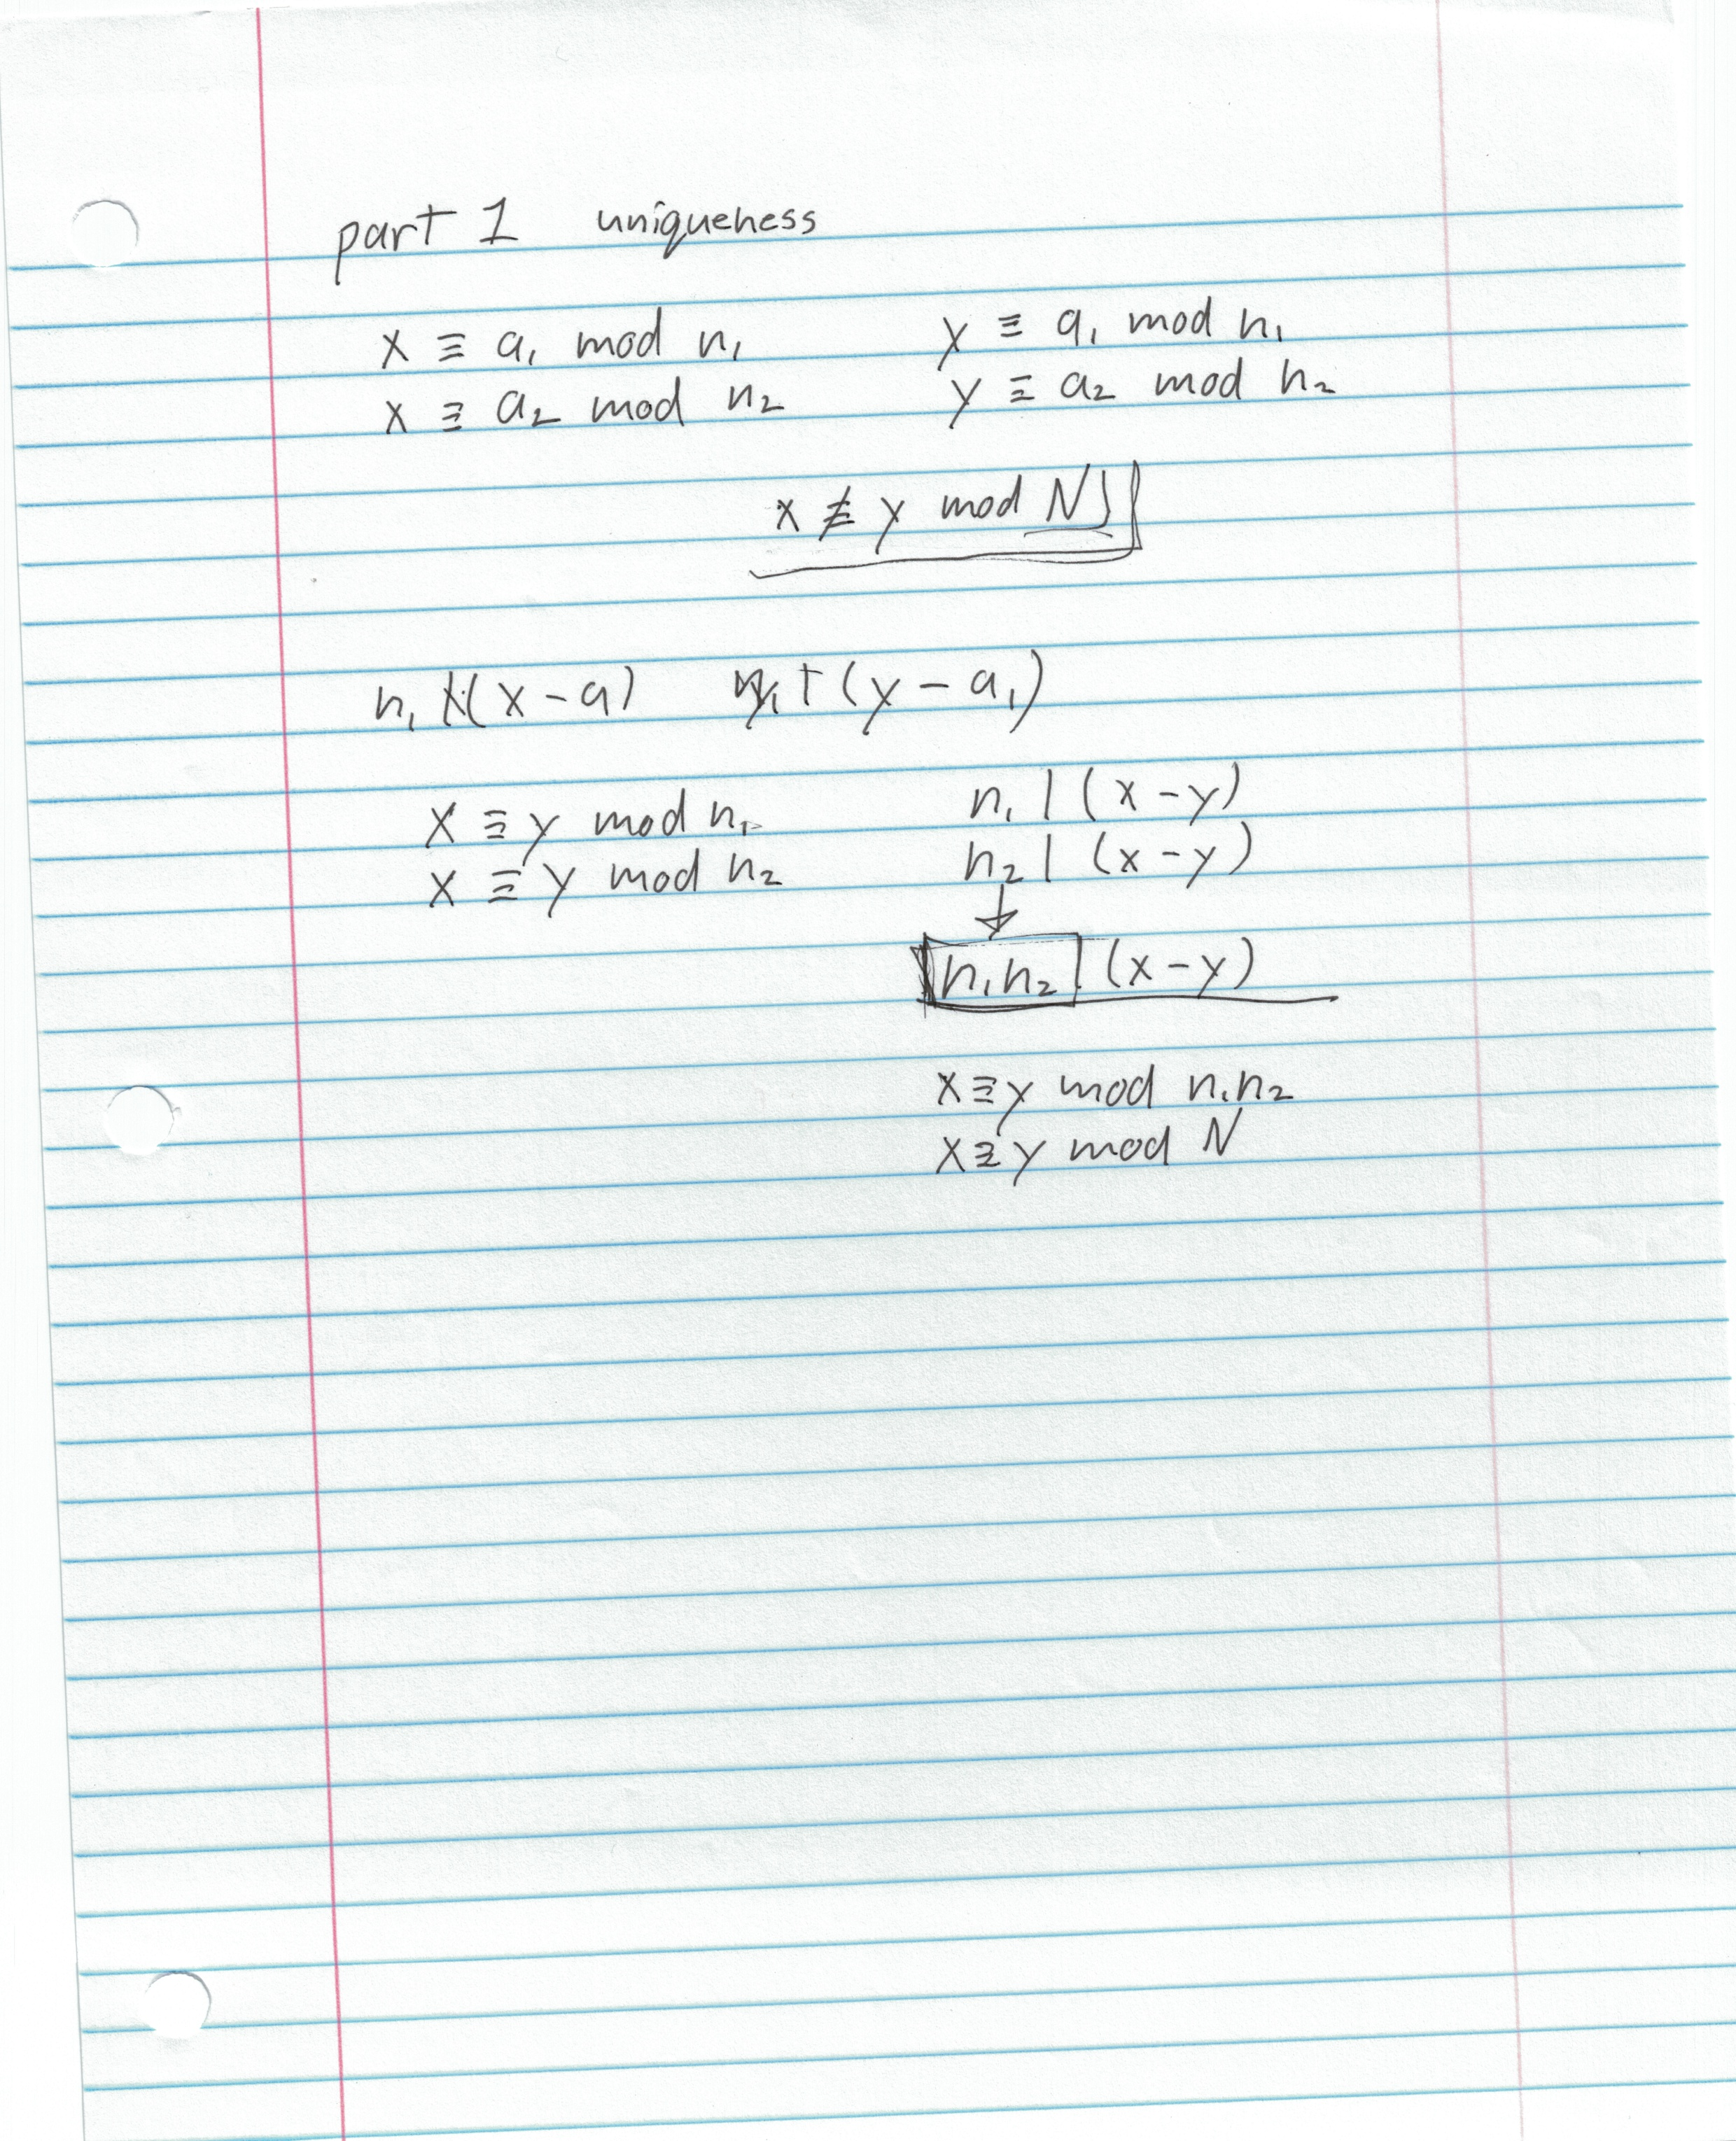
\includegraphics[height=0.8\paperheight]{jacques_page2.jpg}
\end{frame}
\begin{frame}[fragile]
\frametitle{Handwritten CRT Presentation - 3/4}
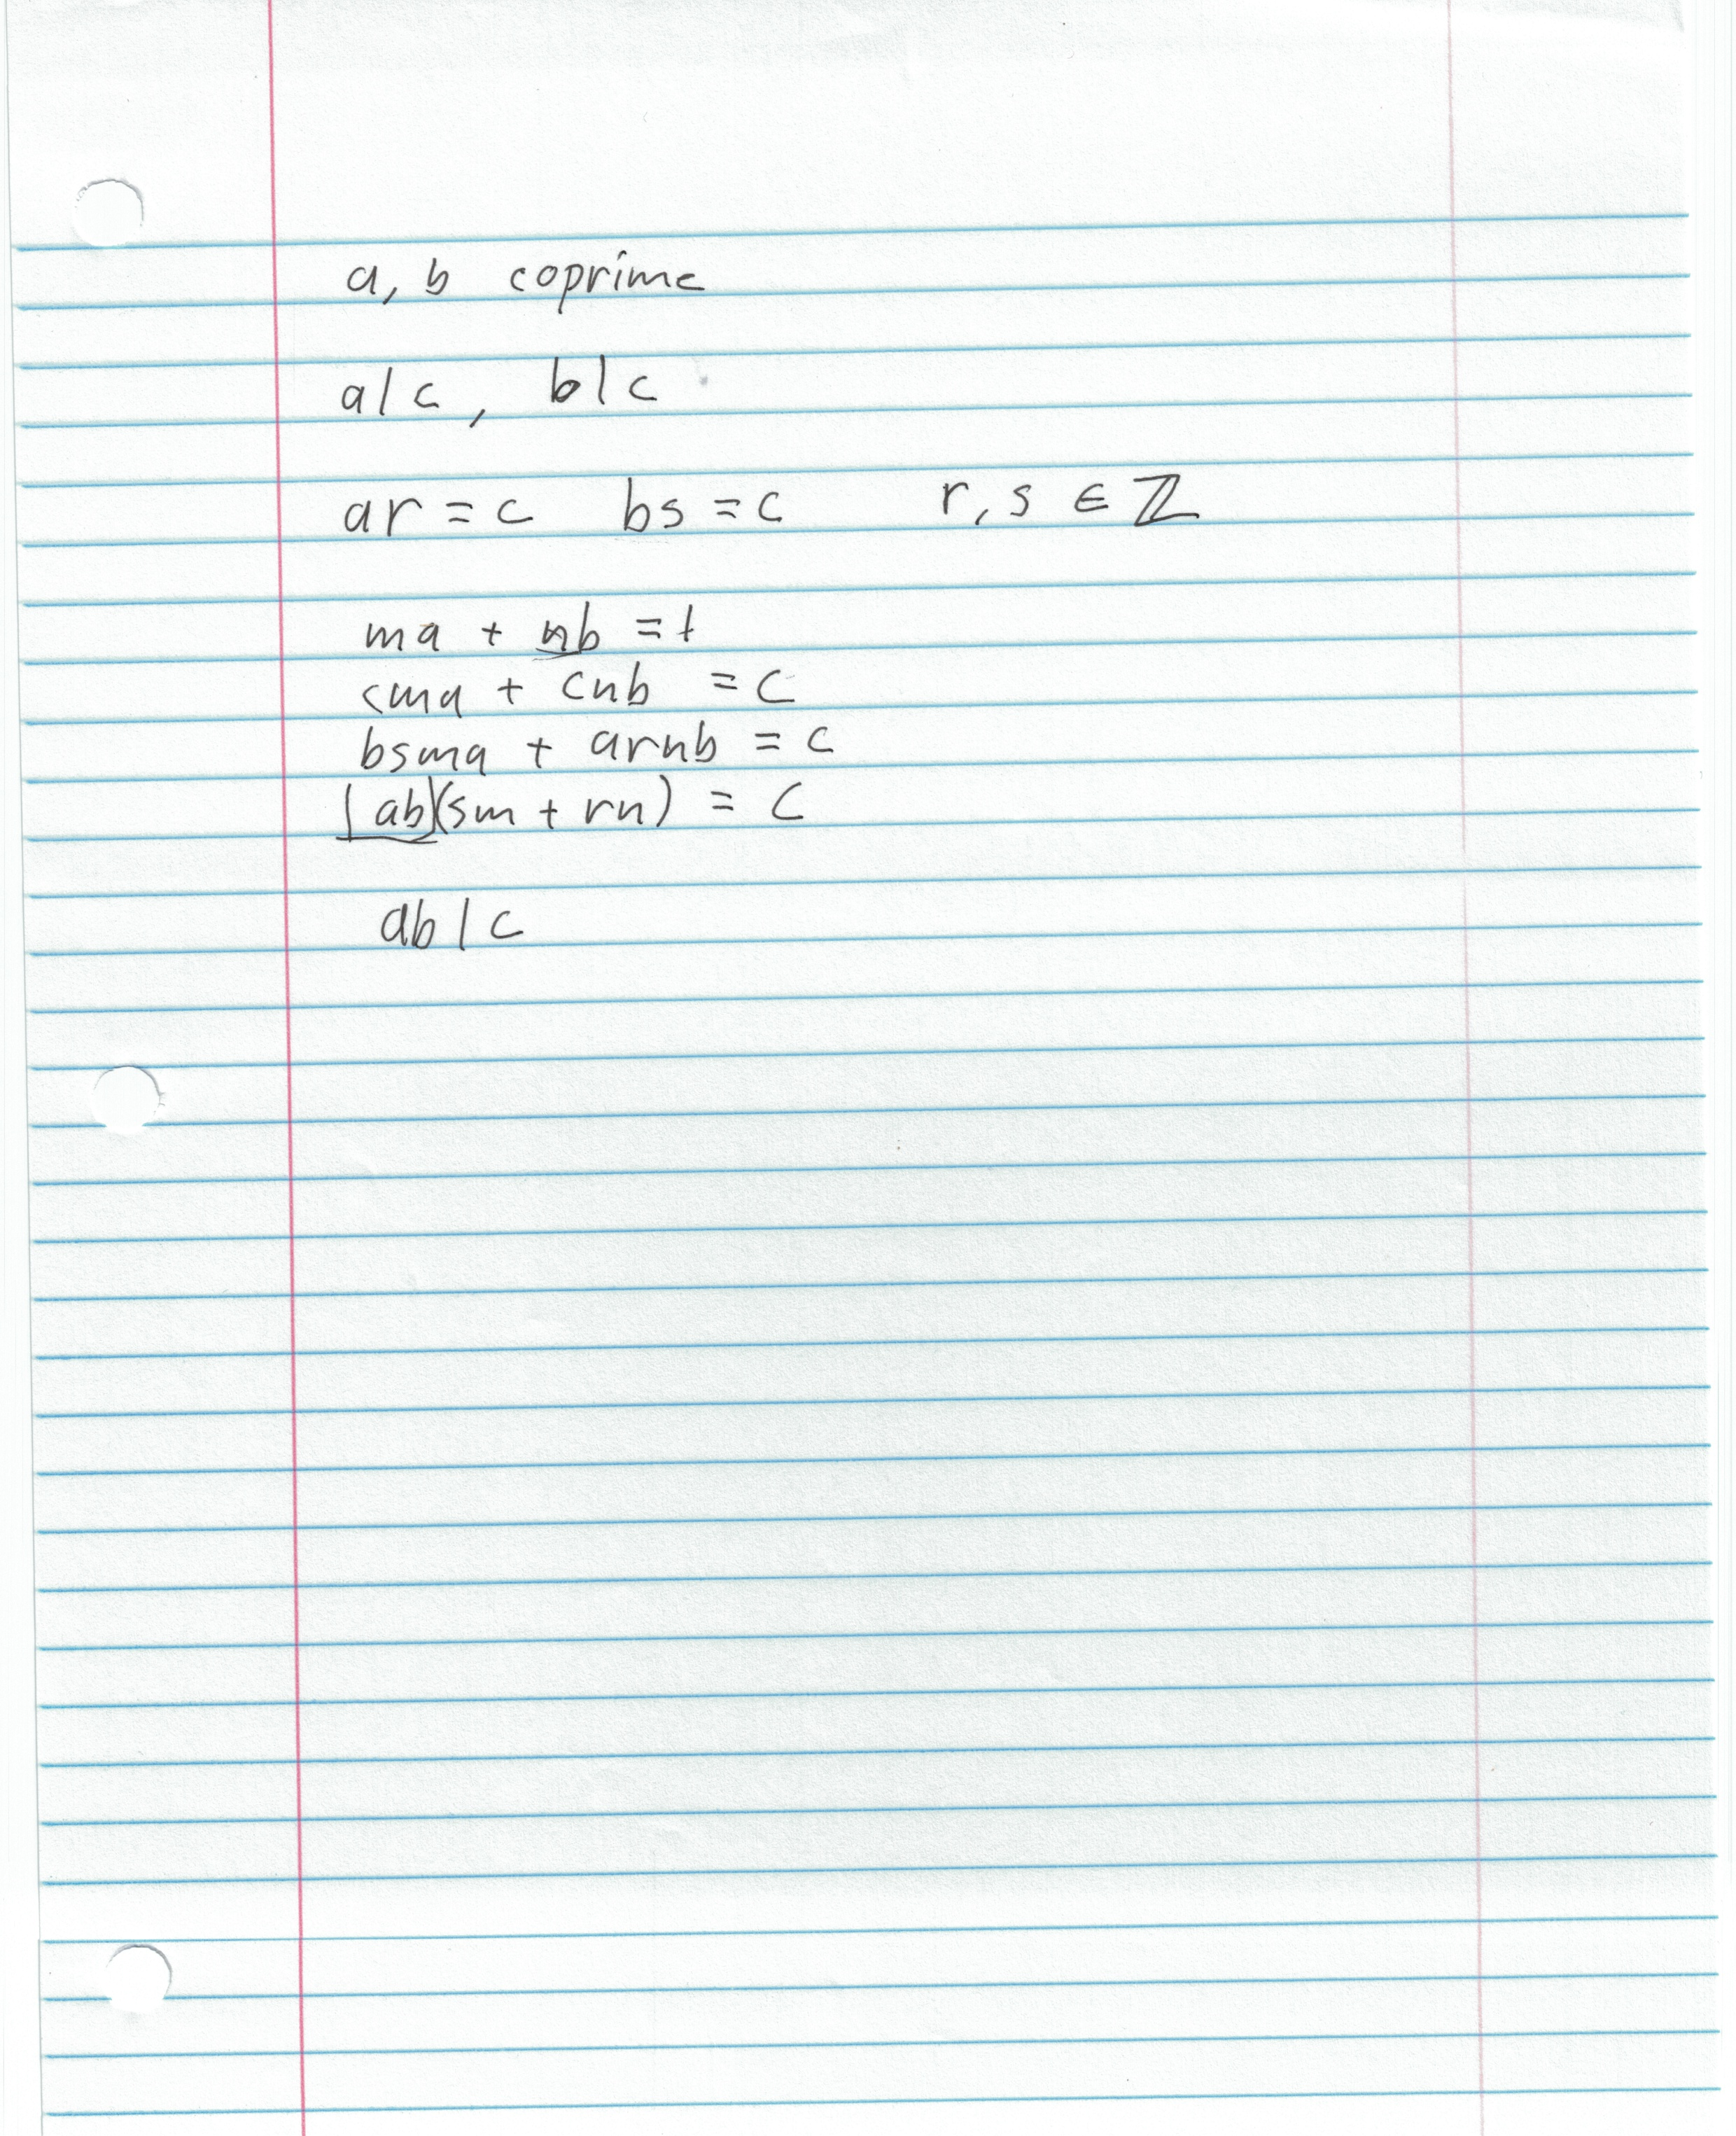
\includegraphics[height=0.8\paperheight]{jacques_page3.jpg}
\end{frame}
\begin{frame}[fragile]
\frametitle{Handwritten CRT Presentation - 4/4}
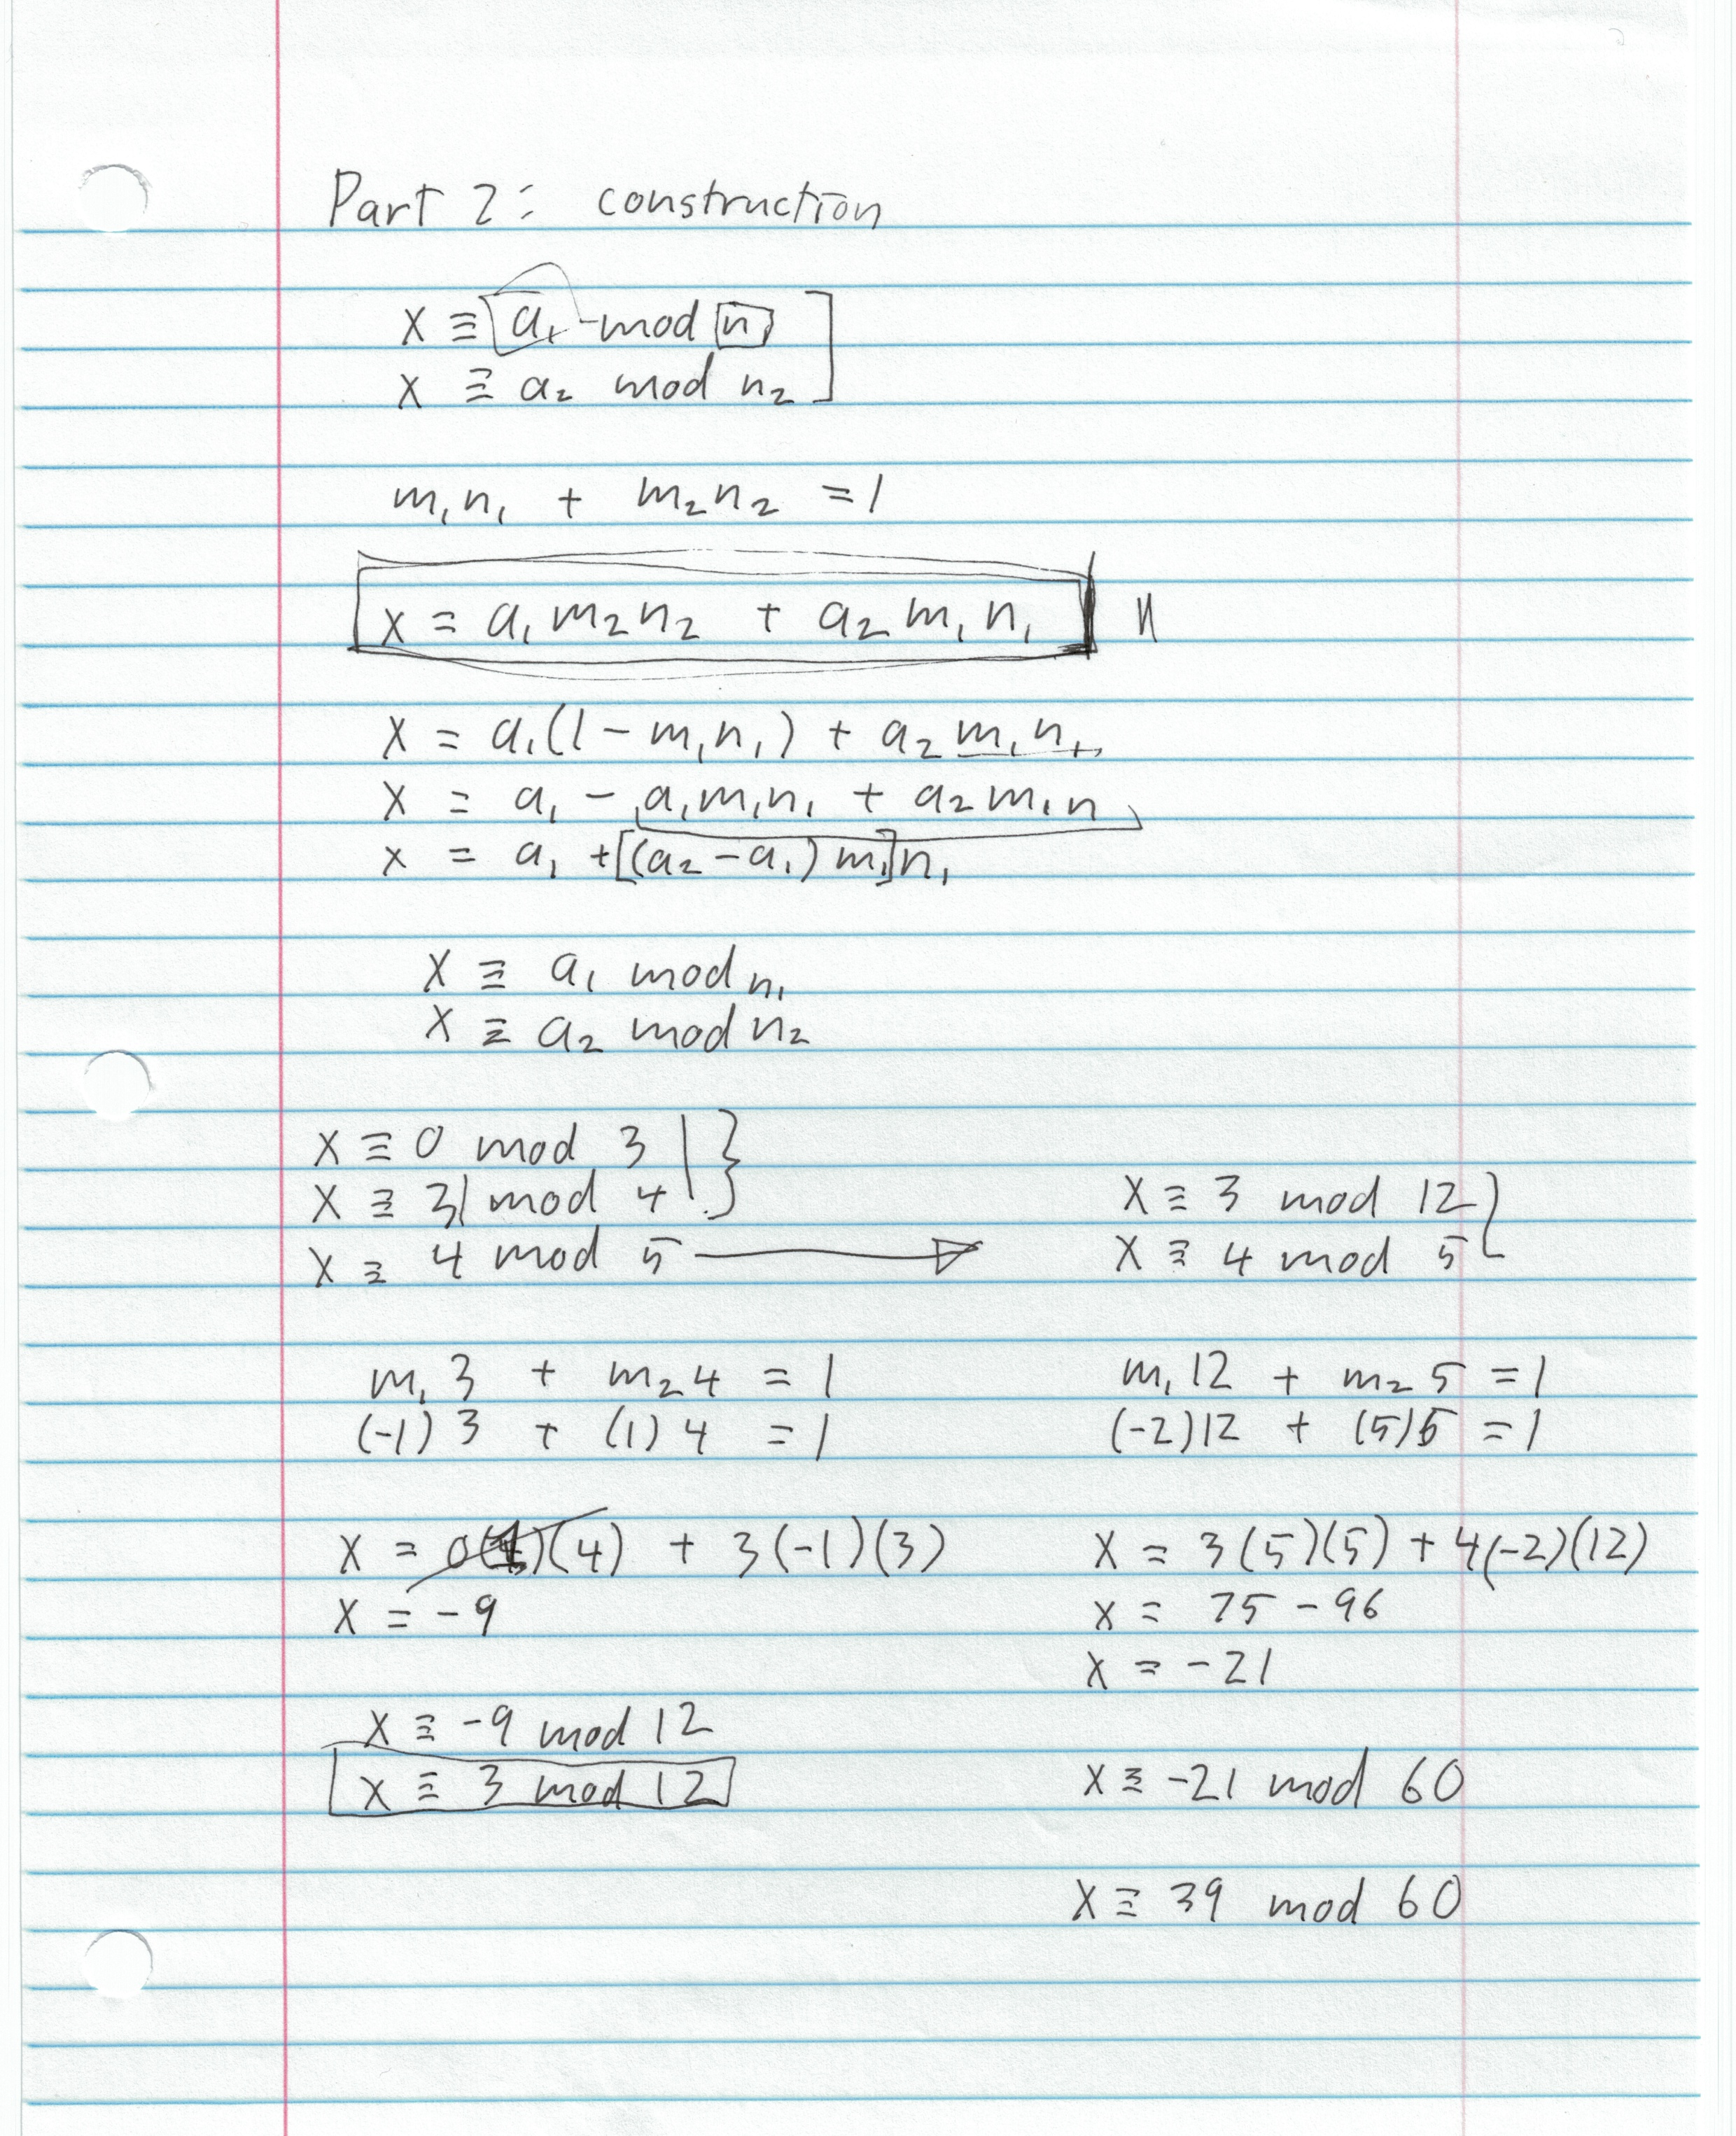
\includegraphics[height=0.8\paperheight]{jacques_page4.jpg}
\end{frame}


\begin{frame}[fragile]
\frametitle{Chinese Remainder Theorem - Statement}
\begin{itemize}
\item $\forall {\color{green}\vec{a}}, {\color{cybercyan}\vec{n}}((\forall i,j(i \neq j \rightarrow {\color{red}\verb|gcd|({\color{cybercyan}n_i, n_j}) = 1})) \rightarrow \exists {\color{cyberpink}x} \forall i({\color{cyberpink}x} \equiv {\color{green}a_i}\hspace{1mm}(\text{mod }{\color{cybercyan}n_i})))$
\item For a system of equations of the form ${\color{cyberpink}x} \equiv {\color{green}a_i}\hspace{1mm}(\text{mod }{\color{cybercyan}n_i})$
\item if each $({\color{cybercyan}n_i, n_j})$ pair are {\color{red}relatively prime}
\item there is a (unique) solution ${\color{cyberpink}x}$ for the system of equations
\end{itemize}
\end{frame}

\begin{frame}[fragile]
\frametitle{Chinese Remainder Theorem - Code}
\begin{itemize}
%\item $\forall \vec{a}, \vec{n}((\forall i,j(i \neq j \rightarrow \verb|gcd|(n_i, n_j) = 1)) \rightarrow \exists x \forall i(x \equiv a_i\hspace{1mm}(\text{mod }n_i)))$
%\item $\forall {\color{green}\vec{a}}, {\color{cybercyan}\vec{n}}((\forall i,j(i \neq j \rightarrow \verb|gcd|({\color{cybercyan}n_i, n_j}) = 1)) \rightarrow \exists {\color{cyberpink}x} \forall i({\color{cyberpink}x} \equiv {\color{green}a_i}\hspace{1mm}(\text{mod }{\color{cybercyan}n_i})))$
\item $\forall {\color{green}\vec{a}}, {\color{cybercyan}\vec{n}}((\forall i,j(i \neq j \rightarrow {\color{red}\verb|gcd|({\color{cybercyan}n_i, n_j}) = 1})) \rightarrow \exists {\color{cyberpink}x} \forall i({\color{cyberpink}x} \equiv {\color{green}a_i}\hspace{1mm}(\text{mod }{\color{cybercyan}n_i})))$
\item
%\VerbatimInput[fontsize=\scriptsize]{crt.py}
\begin{Verbatim}[fontsize=\scriptsize,commandchars=\\\{\}]
from eea import eea
from gmpy import gcd
from itertools import combinations
def crt(eqns):
    assert len(eqns) >= 2
    assert [\textcolor{red}{gcd(\textcolor{cybercyan}{eqns[i][1], eqns[j][1]}) == 1} for (i, j) in combinations(range(len(eqns)), 2)]
    \textcolor{green}{a0}, \textcolor{cybercyan}{n0} = eqns[0]
    \textcolor{green}{a1}, \textcolor{cybercyan}{n1} = eqns[1]
    _, \textcolor{orange}{m0, m1}, _, _ = eea(\textcolor{cybercyan}{n0, n1})
    assert \textcolor{orange}{m0}*\textcolor{cybercyan}{n0} + \textcolor{orange}{m1}*\textcolor{cybercyan}{n1} == 1
    \textcolor{cyberpink}{x} = (\textcolor{green}{a0}*\textcolor{orange}{m1}*\textcolor{cybercyan}{n1} + \textcolor{green}{a1}*\textcolor{orange}{m0}*\textcolor{cybercyan}{n0}) % (\textcolor{cybercyan}{n0} * \textcolor{cybercyan}{n1})
    if len(eqns) > 2:
        \textcolor{cyberpink}{x} = crt([(\textcolor{pink}{x}, \textcolor{cybercyan}{n0}*\textcolor{cybercyan}{n1})]+eqns[2:])
    for (\textcolor{green}{a}, \textcolor{cybercyan}{n}) in eqns:
        assert \textcolor{cyberpink}{x} % \textcolor{cybercyan}{n} == \textcolor{green}{a} % \textcolor{cybercyan}{n}
    return \textcolor{cyberpink}{x}
\end{Verbatim}
% :'<,'>s/n[01]\?/\\textcolor{cybercyan}{\0}/gc
% :'<,'>s/\<m[01]\?\>/\\textcolor{orange}{\0}/gc
% :'<,'>s/\<x\>/\\textcolor{cyberpink}{\0}/gc
\end{itemize}
\end{frame}

\begin{frame}[fragile]
\frametitle{Chinese Remainder Theorem - Example}
\begin{itemize}
\item $\forall {\color{green}\vec{a}}, {\color{cybercyan}\vec{n}}((\forall i,j(i \neq j \rightarrow \verb|gcd|({\color{cybercyan}n_i, n_j}) = 1)) \rightarrow \exists {\color{cyberpink}x} \forall i({\color{cyberpink}x} \equiv {\color{green}a_i}\hspace{1mm}(\text{mod }{\color{cybercyan}n_i})))$
\item ${\color{cyberpink}x} \equiv {\color{green}3} \hspace{1mm}(\text{mod } {\color{cybercyan}5}) \land {\color{cyberpink}x} \equiv {\color{green}4} \hspace{1mm}(\text{mod } {\color{cybercyan}7})$
\item $\verb|eea|({\color{cybercyan}5,7})$ gives us $({\color{orange}3, -2})$ as the Bezout coefficients
\item This tells us that ${\color{orange}3}*{\color{cybercyan}5} + {\color{orange}(-2)}*{\color{cybercyan}7} = 1$
\item CRT gives us that ${\color{cyberpink}x} = {\color{green}3} * {\color{orange}(-2)} * {\color{cybercyan}7} + {\color{green}5} * {\color{orange}3} * {\color{cybercyan}5}$ solves the equation
\end{itemize}
\end{frame}

\begin{frame}[fragile]
\frametitle{CRT Application - Breaking same-message RSA - Theory}
\begin{itemize}
\item Suppose we have
$c_1 \equiv m^3\hspace{1mm}(\text{mod }n_1)$,
$c_2 \equiv m^3\hspace{1mm}(\text{mod }n_2)$, and
$c_3 \equiv m^3\hspace{1mm}(\text{mod }n_3)$.
\item $\verb|crt|([(c_1, n_1), (c_2, n_2), (c_3, n_3)]) \equiv m^3\hspace{1mm}(\text{mod }n_1*n_2*n_3)$
\item Since $n_1*n_2*n_3 > \verb|max|(n_1, n_2, n_3)$, even if $m^3$ wrapped on each of the moduli, it is likely cube-rootable mod the product of the moduli
\end{itemize}
\end{frame}

%>>> ns = [23*29, 19*31, 37*41]
%>>> ns
%[667, 589, 1517]
%>>> pow(190, 3, 1517)
%643
%>>> pow(190, 3)
%6859000
%>>> [pow(190, 3, n) for n in ns]
%[239, 95, 643]
%>>> from crt import crt
%>>> crt([(239, 667),(95, 589),(643, 1517)]
%... )
%4074073199788171
%>>> crt([(239, 667),(95, 589),(643, 1517)]) % (667 * 589 * 1517)
%6859000
%>>> import gmpy
%>>> gmpy.root(crt([(239, 667),(95, 589),(643, 1517)]) % (667 * 589 * 1517), 3)
%(mpz(190), 1)

\begin{frame}[fragile]
\frametitle{CRT Application - Breaking same-message RSA - Example}
\begin{itemize}
\item $\verb|crt|([(c_1, n_1), (c_2, n_2), (c_3, n_3)]) \equiv m^3\hspace{1mm}(\text{mod }n_1*n_2*n_3)$
\item $(c_1, n_1) = (239, 667)$, $(c_2, n_2) = (95, 589)$, $(c_3, n_3) = (643, 1517)$
\item $\verb|crt([(239, 667), (95, 589), (643, 1517)]) == 6859000|$
\item $\sqrt[3]{6859000} = 190$
\end{itemize}
\end{frame}

\begin{frame}[fragile]
\frametitle{CRT Application - Speeding up RSA decryption - Theory}
\begin{itemize}
\item $\verb|encrypt|(m) = \verb|pow|(m, e, n)$, $\verb|decrypt|(c) = \verb|pow|(c, d, n)$
\item If $e = 65537$, it's small and fast to compute with (around 16 bits), but $d$ is around the size of $n$ (2048 bits if $p$ and $q$ are each 1024 bits)
\item $\verb|fastdecrypt|(c) = \verb|crt|([(\verb|pow|(c, d_p, p), p), (\verb|pow|(c, d_q, q), q)])$, where
$e * d_p \equiv 1\hspace{1mm}(\text{mod }p-1)$ and
$e * d_q \equiv 1\hspace{1mm}(\text{mod }q-1)$
\item Works because $\verb|pow|(c, d_p, p) \equiv m\hspace{1mm}(\text{mod }p)$ (and likewise for $q$), so CRT reconstructs $x \equiv m\hspace{1mm}(\text{mod }p*q)$
\item Is faster because $p$ and $q$ are only 1024 bit, so computations mod those are cheaper
\end{itemize}
\end{frame}

\begin{frame}[fragile]
\frametitle{CRT Application - Speeding up RSA decryption - Code}
\begin{itemize}
\item
\begin{Verbatim}[fontsize=\scriptsize]
from codecs import encode
from gmpy import invert, next_prime
from crt import crt
from time import time
import os

p = next_prime(int(encode(os.urandom(4096/8), 'hex'), 16))
q = next_prime(int(encode(os.urandom(4096/8), 'hex'), 16))
n = p * q
e = 65537
d = invert(e, (p-1)*(q-1))
dp = invert(e, p-1)
dq = invert(e, q-1)

msg = int(encode('hello', 'hex'), 16)
s0 = time(); ctxt = pow(msg, e, n); t0 = time()-s0
s1 = time(); m1 = pow(ctxt, d, n); t1 = time()-s1
s2 = time(); m2 = crt([(pow(ctxt, dp, p), p), (pow(ctxt, dq, q), q)]); t2 = time()-s2
assert m1 == m2 == msg
\end{Verbatim}
\end{itemize}
\end{frame}

\begin{frame}[fragile]
\frametitle{Saltstack 2013 e=1 bug}
% RSA e=1 commit from saltstack 0.15.1 release notes
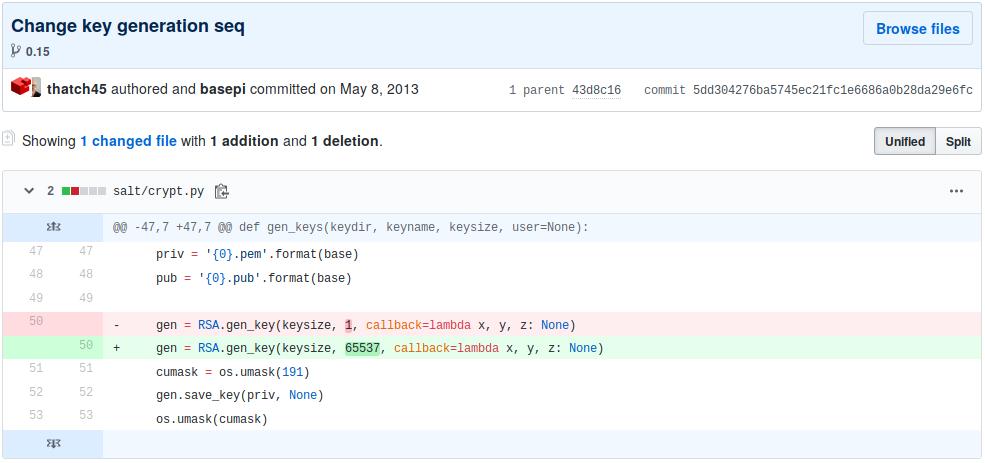
\includegraphics[width=0.9\paperwidth]{saltstack_rsa_diff.png}
\end{frame}


\begin{frame}[fragile]
\frametitle{Resources}
\begin{itemize}
\item \verb|https://en.wikipedia.org/wiki/RSA_(cryptosystem)|
\item \Verb[fontsize=\footnotesize]|https://en.wikipedia.org/wiki/Chinese_remainder_theorem|
\item \verb|https://en.wikipedia.org/wiki/Modular_arithmetic|
\item\Verb[fontsize=\footnotesize]|https://crypto.stanford.edu/~dabo/papers/RSA-survey.pdf|
\item \verb|https://cryptopals.com/|, Sets 5 and 6
\item \Verb[fontsize=\tiny]|https://docs.saltstack.com/en/latest/topics/releases/0.15.1.html#rsa-key-generation-fault|
\end{itemize}
\end{frame}
\end{document}
